\documentclass[11pt, conference]{IEEEtran}
\usepackage{graphicx}
\usepackage{cite}
\usepackage{amsmath}

\twocolumn 

\begin{document}
	\twocolumn[
	\begin{@twocolumnfalse}
		\begin{center}
			\begin{Huge}
				\null
				\vspace{0.6cm}
				\textbf{Distributed Monitoring of the AMS $F_2$ Sketch}
				\vspace{0.6cm}
			\end{Huge}
		\end{center}
  	\end{@twocolumnfalse}
	]


	\subsection{Introduction}

\begin{figure}[!b]
	\center{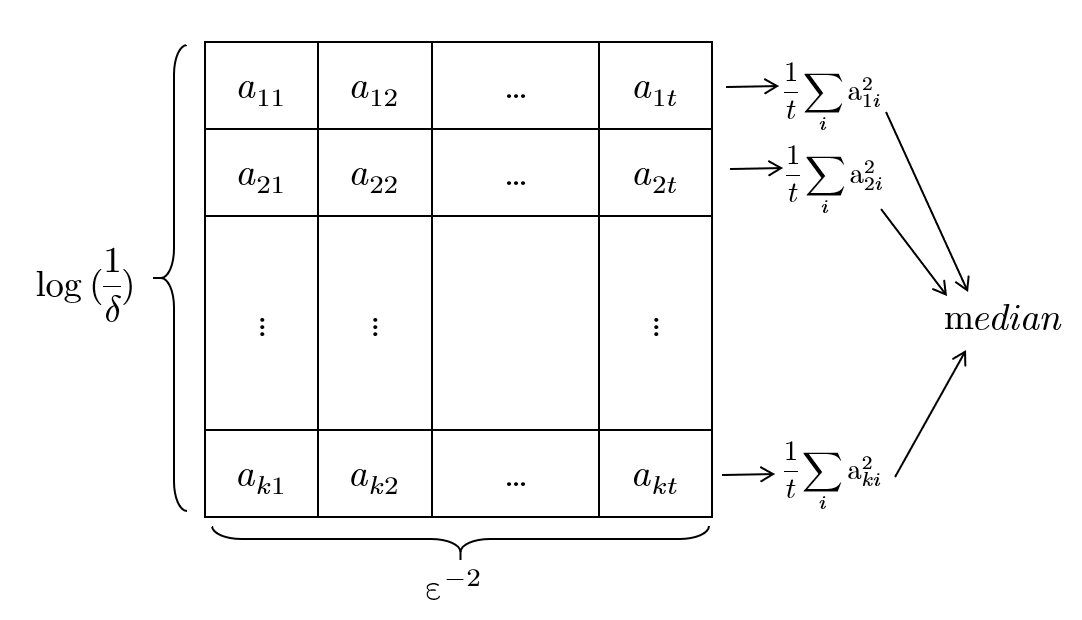
\includegraphics[width=1.0\linewidth]{Pics/AMS_F2.png}}
	\caption{\label{fig:my-label} AMS $F_2$ estimator table.}
\end{figure}	
	
The second frequency moment is a variance-like property of a stream. Let $f_1,...,f_k$ be the frequencies of the k-distinctive items of a stream, then its second moment is $F_2 = {\sum{f_i ^2}}$.

The second moment is applied on ..... anomaly detections ..... (Dani said there's no need to elaborate too much here -- everyone is already convinced that estimating the $F_2$ property of a stream is important)

An efficient unbiased estimator for the value of the second frequency moment of a stream is proposed at \cite{alon1999space}, called an AMS $F_2$ sketch: a four-wise independent hash function is chosen which maps the stream's values to either $+1$ or $-1$ uniformly. The estimator accumulates the summation of all those $+1$'s and $-1$'s; the expected value of the summation squared, equals to the second moment value of the stream.

In order to increase the confidence to $\varepsilon$ and the accuracy to $\delta$, the estimator is duplicated ${\varepsilon ^{-2} log(\frac{1}{\delta})}$ times; then, the estimated $F_2$ value is the median of the averages of every $\varepsilon ^{-2}$ estimators.

Some notations: 
\begin{itemize}
	\item $t=\varepsilon ^{-2}$ -- the number of columns  in the estimators table.
	\item $k=log(\frac{1}{\delta})$ -- the number of rows in the estimators table.
	\item $a_{ij}$ -- the estimator at row $i$ and column $j$.
	\item $r_i = \frac{1}{\sqrt{t}} (a_{i1},a_{i2},...,a_{it})$ -- the vector of estimators at row $i$, normalized.
\end{itemize}

For clarification, the median of the squared norms of the rows, $||r_i||^2$ is the estimated $F_2$.


	\subsection{Monitoring over a dynamic vector}

In order to track the approximation value of the $F_2$ moment, each distributed server maintains its own ${(k \times t)}$ table of estimators.

The point-wise summation of those tables is the estimator table of the global combined stream. So, incorporating the \textit{Convex Bound Method} on the AMS $F_2$ estimator is done by treating the estimator table as the dynamic vector.

	\subsection{Convex Upper Bound}

Applying the Convex Bound Method requires bounding the estimator's function by a convex function from above. Notice that the squaring operation is already convex, and the average operation is linear, so only the median part has to be treated.
Bounding the median function from above, is done by taking the maximum value of half the number of rows -- plus one. Let $k' = {\lfloor 0.5 \cdot k  + 1\rfloor}$; then the maximum of $k'$ arbitrary $||r_i||^2$ values will suffice as an upper-bound; furthermore, the $maximum$ function is convex.

Though, in order to make the bound tight, the convex bound should take into account only the $k'$ minimum $||r_i||^2$ rows at time zero.

Let $i_1 ... i_{k'}$ be the indices of the $r_i$ rows with the minimum norm values at time zero; then, the convex upper bound of the AMS $F_2$ estimator-table is the maximum of the squared norm of those $r_i$ rows. Notice that at time zero, the AMS $F_2$ estimator-table function equals to its upper bound (when k is odd).

	\subsection{Convex Lower Bound}

Bounding the AMS $F_2$ from below is similar to bounding from above. First, the squaring operation of each $a_{ij}$ estimator is bound from below by a tangent plane. Then, since the average operation is linear -- it doesn't change, and instead of 'convexising' the median operation by the maximum function, it is bound by the minimum function. Additionally, like the upper bound, in order to make the bound tight, only the $k'$ rows with the minimum value at time zero are taken.

	\subsection{$L_2$ Distance to Upper Bound}

Calculating the $L_2$ distance to the convex bound is different whether the point is from inside the convex bound or outside the convex bound (** note: should we define what's the definition of 'inside' and what's the definition of 'outside' or is it trivial? **). We'll show how to calculate the distance relative to the convex upper bound, denote, $c$, whereas, calculating the distance to the lower concave bound is quite similar.

		\subsubsection{Distance From Inside}
	
Let $A$ be the estimator table and $c$ the convex upper bound of the AMS $F_2$ function. Let $T$ be the threshold and assume ${c(A) < T}$. Calculating the $L_2$ distance to the surface of the convex ${\{v \ |\ c(v) = T\}}$, means we'd like to find a vector v where ${c(A+v)=T}$ while minimizing $||v||_2$. Since the convex surface is a maximum of the squared norm of some rows of $A$, the minimum $||v||_2$ would be all zeros, except of at the row of the largest norm. Mark $r_m$ to be the row with the maximum norm, while ${m \in \{i_1 ... i_{k'}\}}$. $v$'s values at the indices of row $r_m$ would be as the distance to the norm squared function. Precisely:

\[
    v_{ij}= 
\begin{cases}
    a_{ij} (\frac{\sqrt{T}}{||r_m||}-1),& \text{if } i = m \\
    0,                                  & \text{otherwise}
\end{cases}
\]


		\subsubsection{Distance From Outside}

Let $A$ be the estimator table, $T$ the threshold, $c$ the convex bound and $v$ the distance vector we'd like to find. Assume ${c(A) > T}$. Since the convex function is a maximum of the $||r_i||^2$, the minimum $||v||_2$ would be all zeros, except at the rows where $||r_i||^2 > T$ when ${i \in \{i_1 ... i_{k'}\}}$. When a row's squared norm value is above $T$, we'd decrease it like a distance to the norm squared function. Precisely:
\[
    v_{ij}= 
\begin{cases}
    a_{ij} (\frac{\sqrt{T}}{||r_m||}-1),& \text{if } i \in \{i_1 ... i_{k'}\} \wedge ||r_i||^2 > T  \\
    0,                                  & \text{otherwise}
\end{cases}
\]


	\subsection{An Alternative Norm-Metric}

Unfortunately, since AMS $F_2$ convex upper-bound behaves as a maximum function, the $L_2$ norm to the surface tends to be heavier when crossing the threshold. Thereby, it's predicted to have poor performance when applied in The Distance Scheme.

In order to engineer an alternative norm-metric for the AMS $F_2$ estimator table, we'll exploit the maximum-behaviour of the convex bound. Thus, we'll fuse the $L_\infty$ norm with the $L_2$ norm of the rows.

Let $A$ be an estimator table of size $k \times t$ and ${r_{i_1},...,r_{i_{k'}}}$ be the rows with minimum norm at time zero. Define the norm of $A$ to be:

$$\widetilde{norm}(A) = \max\limits_{j} {(||r_{i_j}||)}$$

Proving that $\widetilde{norm}$ is a norm is easy to prove. With that special norm, calculating the distance to the surface of the convex bound would require only a change in the row $r_i$ with the maximum norm value out of $i \in \{i_1,...,,i_{k'}\}$, both from the inside and from the outside. Thus, the disadvantage of the classic $L_2$ norm is avoided. Let  $r_m$ be the row out of ${r_{i_1},...,r_{i_{k'}}}$ with the maximum norm, then, the distance vector to the surface is as follows, both from inside the convex bound, and outside the convex bound.:

\[
    v_{ij}= 
\begin{cases}
    a_{ij} (\frac{\sqrt{T}}{||r_m||}-1),& \text{if } i = m \\
    0,                                  & \text{otherwise}
\end{cases}
\]

	\bibliography{AMS_F2}{}
	\bibliographystyle{plain}


\end{document}